%%% Класс документа
\documentclass[a4paper,14pt]{article}

%%% Работа с русским языком
\usepackage{cmap}					% поиск в PDF
\usepackage[warn]{mathtext}
\usepackage[T2A]{fontenc}			% кодировка
\usepackage[utf8]{inputenc}			% кодировка исходного текста
\usepackage[english,russian]{babel}	% локализация и переносы
\usepackage{mathtext} 				% русские буквы в формулах
\usepackage{csvsimple}              % for tabular from csv loading
\usepackage{indentfirst}            % indent after sections
%\usepackage{minipage}

%%% Дополнительная работа с математикой
\usepackage{amsmath,amsfonts,amssymb,amsthm,mathtools} % AMS
\usepackage{icomma} % "Умная" запятая: $0,2$ --- число, $0, 2$ --- перечисление

%%% Номера формул
%\mathtoolsset{showonlyrefs=true} % Показывать номера только у тех формул, на которые есть \eqref{} в тексте.
%\usepackage{leqno} % Немуреация формул слева

%%% Шрифты
\usepackage{euscript}	 % Шрифт Евклид
\usepackage{mathrsfs} % Красивый матшрифт

%%% Свои команды
\DeclareMathOperator{\sgn}{\mathop{sgn}}

%%% Перенос знаков в формулах (по Львовскому)
\newcommand*{\hm}[1]{#1\nobreak\discretionary{}
{\hbox{$\mathsurround=0pt #1$}}{}}

%%% Работа с картинками
\usepackage{graphicx}  % Для вставки рисунков
\graphicspath{{images/}{images2/}}  % папки с картинками
\setlength\fboxsep{3pt} % Отступ рамки \fbox{} от рисунка
\setlength\fboxrule{1pt} % Толщина линий рамки \fbox{}
\usepackage{wrapfig} % Обтекание рисунков и таблиц текстом

%%% Работа с таблицами
\usepackage{array,tabularx,tabulary,booktabs} % Дополнительная работа с таблицами
\usepackage{longtable}  % Длинные таблицы
\usepackage{multirow} % Слияние строк в таблице

%%% Теоремы
\theoremstyle{plain} % Это стиль по умолчанию, его можно не переопределять.
%\newtheorem{theorem}{Теорема}[section]
%\newtheorem{proposition}[theorem]{Утверждение}
 
%\theoremstyle{definition} % "Определение"
%\newtheorem{corollary}{Следствие}[theorem]
%\newtheorem{problem}{Задача}[section]
 
%\theoremstyle{remark} % "Примечание"
%\newtheorem*{nonum}{Решение}

%%% Программирование
\usepackage{etoolbox} % логические операторы

%%% Страница
\usepackage{extsizes} % Возможность сделать 14-й шрифт
\usepackage{geometry} % Простой способ задавать поля
	\geometry{top=25mm}
	\geometry{bottom=35mm}
	\geometry{left=35mm}
	\geometry{right=20mm}
	
%%% Колонтитулы
%\usepackage{fancyhdr}
 	%\pagestyle{fancy}
 	%\renewcommand{\headrulewidth}{0mm}  % Толщина линейки, отчеркивающей верхний колонтитул
 	%\lfoot{Нижний левый}
 	%\rfoot{Нижний правый}
 	%\rhead{Верхний правый}
 	%\chead{Верхний в центре}
 	%\lhead{Верхний левый}
 	% \cfoot{Нижний в центре} % По умолчанию здесь номер страницы
 	
%%% Интерлиньяж
%\usepackage{setspace}
%\onehalfspacing % Интерлиньяж 1.5
%\doublespacing % Интерлиньяж 2
%\singlespacing % Интерлиньяж 1

%%% Гиперссылки
\usepackage{hyperref}
\usepackage[usenames,dvipsnames,svgnames,table,rgb]{xcolor}
\hypersetup{				% Гиперссылки
    unicode=true,           % русские буквы в раздела PDF
    pdftitle={Заголовок},   % Заголовок
    pdfauthor={Автор},      % Автор
    pdfsubject={Тема},      % Тема
    pdfcreator={Создатель}, % Создатель
    pdfproducer={Производитель}, % Производитель
    pdfkeywords={keyword1} {key2} {key3}, % Ключевые слова
    colorlinks=true,       	% false: ссылки в рамках; true: цветные ссылки
    linkcolor=red,          % внутренние ссылки
    citecolor=green,        % на библиографию
    filecolor=magenta,      % на файлы
    urlcolor=cyan           % на URL
}

%%% Другие пакеты
\usepackage{lastpage} % Узнать, сколько всего страниц в документе.
\usepackage{soul} % Модификаторы начертания
\usepackage{csquotes} % Еще инструменты для ссылок
%\usepackage[style=authoryear,maxcitenames=2,backend=biber,sorting=nty]{biblatex}
\usepackage{multicol} % Несколько колонок
\usepackage{multirow} % Несколько строк

%%% Шрифты
%\renewcommand{\familydefault}{\sfdefault} % Начертание шрифта


%%% Работа с библиографией
%\usepackage{cite} % Работа с библиографией
%\usepackage[superscript]{cite} % Ссылки в верхних индексах
%\usepackage[nocompress]{cite} % 
%\usepackage{csquotes} % Еще инструменты для ссылок


%%% Tikz
\usepackage{tikz} % Работа с графикой
\usepackage{pgfplots} % Работа с pgf
\usepackage{pgfplotstable}
\usepackage{upgreek}

%%% Дополнительные пакеты для tikz
%\usepgfplotslibrary{dateplot} % Возможность подписания дат
\pgfplotsset{compat=1.5}
% \newcommand{\eqdef}{\stackrel{\mathrm{def}}{=}}
% \newcommand{\ryad}{\sum\limits^{\infty}_{k = 0}}

% \newcommand{\R}{\mathbb{R}}
% \newcommand{\N}{\mathbb{N}}
% \newcommand{\series}{\sum\limits_{k=1}^{\infty}}
% \newcommand{\useries}{\sum\limits_{k=1}^{\infty} u_k}
% \newcommand{\useriesl}{\sum\limits_{k=1}^{\infty} u_k < \infty}
% \newcommand{\useriese}{\sum\limits_{k=1}^{\infty} u_k = \infty}
% \newcommand{\auseries}{\sum\limits_{k=1}^{\infty} |u_k|}
% \newcommand{\auseriesl}{\sum\limits_{k=1}^{\infty} |u_k| < \infty}
% \newcommand{\auseriese}{\sum\limits_{k=1}^{\infty} |u_k| = \infty}
% \newcommand{\sn}{\sum\limits_{k=1}^{n} u_k}

% \renewcommand {\ge}{\geqslant}
% \renewcommand {\le}{\leqslant}
% \renewcommand {\geq}{\geqslant}
% \renewcommand {\leq}{\leqslant}
% \renewcommand {\epsilon}{\varepsilon}

\begin{document}
    \newcommand{\HRule}{\rule{\linewidth}{0.7mm}} % Defines a new command for the horizontal lines, change thickness here
	
	\begin{center}
		\large\textbf{Московский Физико-Технический Институт}\\ % Name of your university/college
		\large\textbf{(государственный университет)}
	
		\vfill
		
		\Large Лабораторная работа по курсу общей физики № *labnum*\\[0.5cm] % Preambule of your document title
		
		
		\HRule
		\\[0.4cm]
		{ \huge \bfseries *name of your labwork*}% Title of your document
		\\[0.4cm] 
		\HRule
		\\[0.5cm]
		
		\ \\
	\textbf{\large Автор:} \\	
	\large *your name* *groupname*\\ % Your name and something more, your group num for example
		\vfill
		\hspace*{-0.8 cm}
\includegraphics[width=100 pt]{frkt_logo}\\ % logo of your  company/university/college
		\large Долгопрудный, 2021 % location and year
	\end{center}

\newpage
\setcounter{page}{2}
\fancyfoot[c]{\thepage}
\fancyhead[L] {Работа № *labnum*} % some information in page header
\fancyhead[R]{}

    \section*{Задание 1. Делитель напряжения.}

    \begin{figure}[h!]
        \centering
        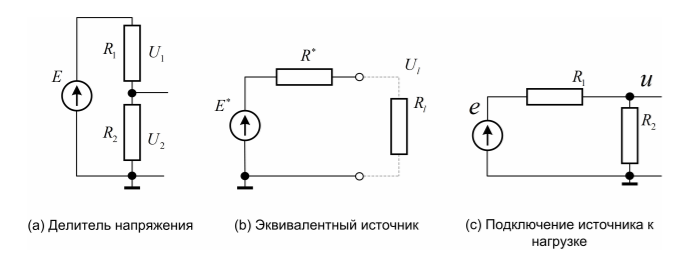
\includegraphics[scale = 1]{делитель_напряжения.png}
        \caption{Делитель напряжения}
        %\label{}
    \end{figure}

    \noindent Напряжение питания $E = $ V, а выходное напряжение $E^* = $ V. 
    Возмем $R_1 = $ kOm, тогда вычислим $R_2$ по формуле:
    \begin{equation*}
        \frac{E - E^*}{R_1} = \frac{E^*}{R_2}
    \end{equation*} 
    Таким образом, получаем $R_2 = $ kOm.

    \noindent Измеряем полученное выходное напряжение при помощи АЦП в
    генераторе. Получаем $E^*_{\text{изм}} = $ V.

    \noindent Чтобы померить эквивалентное сопротивление источника, используем метод двух нагрузок. 
    Возьмём резистор $R_l = $ kOm. 
    При помощи того же АЦП меряем напряжение на нагрузке $U_l = $ V.
    Найдем эквивалентное сопративление по формуле:
    \begin{equation*}
        \frac{E^* - U_l}{R^*} = \frac{U_l}{R_l}
    \end{equation*} 
    Отсюда получаем $R^* = $ kOm.

    \noindent Подаём на вход синусоидальное напряжение $e$. 
    Найдём коэффициент передачи:
    \begin{equation*}
        K = \frac{u}{e}
    \end{equation*} 
    В результате получаем, что эффективные $e = $ V, $u = $ V, то есть $K = $.
    Теоретический расчет дает $K_{\text{теор}} = $ю

    \section*{Задание 2. Паралелльный сумматор.}

    \begin{figure}[h!]
        \centering
        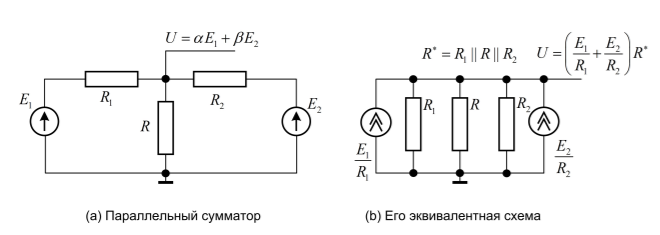
\includegraphics[scale = 1]{сумматор.png}
        \caption{Паралелльный сумматор}
        %\label{}
    \end{figure}

    \noindent Из условия $\alpha = 0.4$, $\beta = 0.2$.

    \[ \frac{R_2}{R_1} = \frac{\alpha}{\beta} \]
    \[ \alpha + \beta = 0.6 = \frac{1}{1 + \frac{R_1 || R_2}{R}} \]

    \noindent Таким образом, получаем: $R_1 : R_2 : R = 1 : 2 : 1$.

    \noindent Собираем схему и смотрим на осциллографе постоянную и 
    переменную составляющую (либо поочередно закорачиваем источники). 
    Получаем, что $U_{=} = $ V, $U_{\approx} = $ V. Отсюда вычисляем $\alpha = $, $\beta = $.

    \noindent Измеряем по эквивалентное сопротивление по методу 2 нагрузок.
    Возьмём за нагрузку резистор $R_l = $ kOm. Тогда полученное напряжение
    $U^l_{=} = $ V, $U^l_{\approx} = $ V.
    Итоговое сопротивление получается равным $R^* = $ kOm. Расчетное сопративление
    $R^*_{\text{расч}} = R_1 || R_2 || R =  $ kOm.

    \section*{Задание 3. H-параметры.}

    \noindent Проверим теоритическую зависимость. Если $U_2 = 0$, то
    \[ h_{11} = R_1 + R_2 || R_3 \]
    \[ h_{21} = \frac{R_3}{R_2 + R_3} \]
    Если $I_1 = 0$, то
    \[ h_{12} = \frac{U_1}{U_2} = - \frac{R_3}{R_2 + R_3} \]
    \[ h_{22} = \frac{I_2}{U_2} = \frac{1}{R_2 + R_3} \] 

    Проведем измерения в Micro-Cap.
    \begin{figure}[h!]
        \centering
        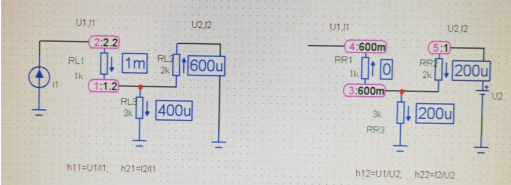
\includegraphics[scale = 1]{Hparams.png}
        \caption{H-параметры}
        %\label{}
    \end{figure}

    \[ h_{11} = \frac{U_1}{I_1} = \frac{2.2 ~ V}{1 ~ mA} = 2.2 ~ kOm \]
    \[ h_{12} = \frac{I_2}{I_1} = \frac{-600 ~ mkA}{1 ~ mA} = -0.6 \]
    \[ h_{21} = \frac{U_1}{U_2} = \frac{600 ~ mV}{1 ~ V} = 0.6 \]
    \[ h_{22} = \frac{I_1}{U_2} = \frac{200 ~ mkA}{1 mA} = 0.2 ~ kOm^{-1} \]

    \noindent А так как сопротивление резисторов $R_1 = 1$ kOm, $R2 = 2$ kOm,
    $R3 = 3$ kOm, то легко проверить, что теоритическая связь даёт тот же
    результат.

    \section*{Задание 4. Звезда и Треугольник.}

    \noindent Верность теоретической зависимость аналогично предыдущему 
    заданию можно найти из закона Ома в случаях, когда $I_1 = 0$ и $I_2 = 0$.
    Если сопротивления звезды равны $R_1 = 1$ kOm, $R_2 = 2$ kOm, 
    $R_3 = 3$ kOm, то пересчитав в параметры треугольника получим:
    $R_{13} = 5.5$ kOm, $R_{12} = 11/3$ kOm, $R_{23} = 11$ kOm.

    \newpage
    
    \noindent Проведём измерения в Micro-Cap.
    \begin{figure}[h!]
        \centering
        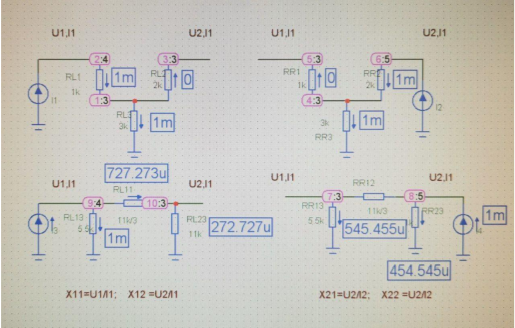
\includegraphics[scale = 1]{triangle.png}
        \caption{Звезда и треугольник}
        %\label{}
    \end{figure}

    \[ X_{11} = \frac{U_1}{I_1} = \frac{4 ~ V}{1 ~ mA} = 4 ~ kOm \]
    \[ X_{12} = \frac{U_1}{I_2} = \frac{3 ~ V}{1 ~ mA} = 3 ~ kOm \]
    \[ X_{21} = \frac{U_2}{I_1} = \frac{3 ~ V}{1 ~ mA} = 3 ~ kOm \]
    \[ X_{22} = \frac{U_2}{I_2} = \frac{5 ~ V}{1 ~ mA} = 5 ~ kOm \]

    \noindent Зная значения резистров, нетрудно проверить справедливость полученных данных.

    \begin{equation*}
        \left(
        \begin{array}{c}
            U_1\\
            U_2
        \end{array}
        \right) =
        \left(
        \begin{array}{cc}
            X_{11} & X_{12}\\
            X_{21} & X_{22}
        \end{array}
        \right)
        \left(
        \begin{array}{c}
            I_1\\
            I_2
        \end{array}
        \right) =
        \left(
        \begin{array}{cc}
            R_1 + R_3 & R_3      \\
            R_3       & R_2 + R_3
        \end{array}
        \right)
        \left(
        \begin{array}{c}
            I_1\\
            I_2
        \end{array}
        \right) 
    \end{equation*}

    \section*{Задание 5. Лестничные структуры.}

    \noindent Рассмотрим лестничные структуры.
    \begin{figure}[h!]
        \centering
        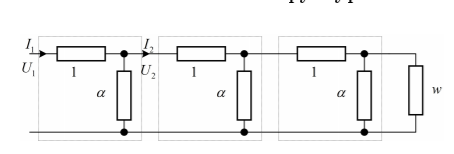
\includegraphics[scale = 1]{лестничные_структуры.png}
        \caption{Лестничные структуры.}
        %\label{}
    \end{figure}

    \noindent Исследуем напряжения в узлах и токи в ветвях для различных случаев.

    \begin{enumerate}
        \item $\alpha = 2,  ~ \gamma = \frac{1}{2}, ~ \omega = 2 ~ kOm$
        \item $\alpha = 6,  ~ \gamma = \frac{2}{3}, ~ \omega = 3 ~ kOm$
        \item $\alpha = 12, ~ \gamma = \frac{3}{4}, ~ \omega = 4 ~ kOm$
        \item $\alpha = 1,  ~ \gamma = \frac{\sqrt{5} - 1}{\sqrt{5} + 1} \approx 0.38, ~ \omega = \frac{1 + \sqrt{5}}{2} \approx 1.618 ~ kOm$
    \end{enumerate}

    \section*{Задание 5. ЦАП.}

    \noindent Снимем зависимость напряжения OUT от двоичного кода ($X_3$, $X_2$, $X_1$, $X_0$).

    \begin{enumerate}
        \item $(0, 0, 0, 0) = 0 ~ V$
        \item $(0, 0, 0, 1) = 1 ~ V$
        \item $(0, 0, 1, 0) = 2 ~ V$
        \item $(0, 0, 1, 1) = 3 ~ V$
        \item $(0, 1, 0, 0) = 4 ~ V$
        \item $(1, 0, 0, 0) = 8 ~ V$
        \item $(1, 1, 0, 1) = 13 ~ V$
        \item $(1, 1, 1, 1) = 15 ~ V$
    \end{enumerate}

\end{document}